\documentclass{article}
\usepackage[utf8]{inputenc}
\usepackage{url}
\usepackage{amsmath,amsthm,enumitem}
\usepackage{graphicx}
\usepackage{lscape}
\usepackage{geometry}
\usepackage{color}
\usepackage{float}
\usepackage{listings}
\usepackage{amssymb}
\usepackage{enumitem}
\usepackage{verbatim}
\usepackage{algpseudocode} 
\usepackage{algorithm}  
\usepackage{algorithmicx}  
\usepackage{hyperref}
\usepackage{authblk}
\geometry{left=2.5cm,right=2.5cm,top=2cm,bottom=2.5cm} 
\renewcommand{\baselinestretch}{1.5}
\newcommand\numberthis{\addtocounter{equation}{1}\tag{\theequation}}
\setcounter{MaxMatrixCols}{20}

\title{Solving Large Systems of Linear Equations}
\author{Haocheng Dai }
\date{}
\DeclareUnicodeCharacter{2212}{-}

\begin{document}
\maketitle
\section{Quadratic Form}
Given $A$ (positive-definite and symmetric) and $ b$, our target is to find a $x_*$ such that
\begin{equation}
    Ax_*= b.
\end{equation}

If we want to find the solution of Eq.(1), we can just try to minimize the convex function $f(x)$:
\begin{equation}
   f( x)=\frac{1}{2} x^TA x- x^T b,\text{   where } \nabla f( x)=\frac{1}{2}A^Tx+\frac{1}{2}Ax- b.
\end{equation}

As $A$ is symmetric, the gradient reduces to
\begin{equation*}
    \nabla f(x)=Ax-b
\end{equation*}
Because $A$ is positive-definite, the surface defined by $f(x)$ is shaped like a paraboloid bowl, which is illustrated by Figure~\ref{fig:quadratic}. Only if $f(x)$ is a convex function, we can find a stationary point.

Gradient is the direction in which the function rises. And here are another two definitions we should memorize through out the note:
\begin{itemize}
    \item \makebox[2cm][l]{\textbf{Error}}  \makebox[4cm][l]{$e_i=x_i-x_*$} is a vector indicates how far we are from the solution $x_*$.
    \item \makebox[2cm][l]{\textbf{Residual}} \makebox[4cm][l]{$r_i=b-Ax_i=-\nabla f(x_i)$} is a vector indicates how far we are form the correct value $b$.
\end{itemize}

And the relationship between error and residual is 
\begin{equation}
    r_i=-Ae_i.
\end{equation}

Remember whenever we read \textbf{residual}, think \textbf{“direction of steepest descent"}; whenever read \textbf{gradient} , think \textbf{“direction of steepest ascent"}.
\begin{figure}[H]
   \centering
   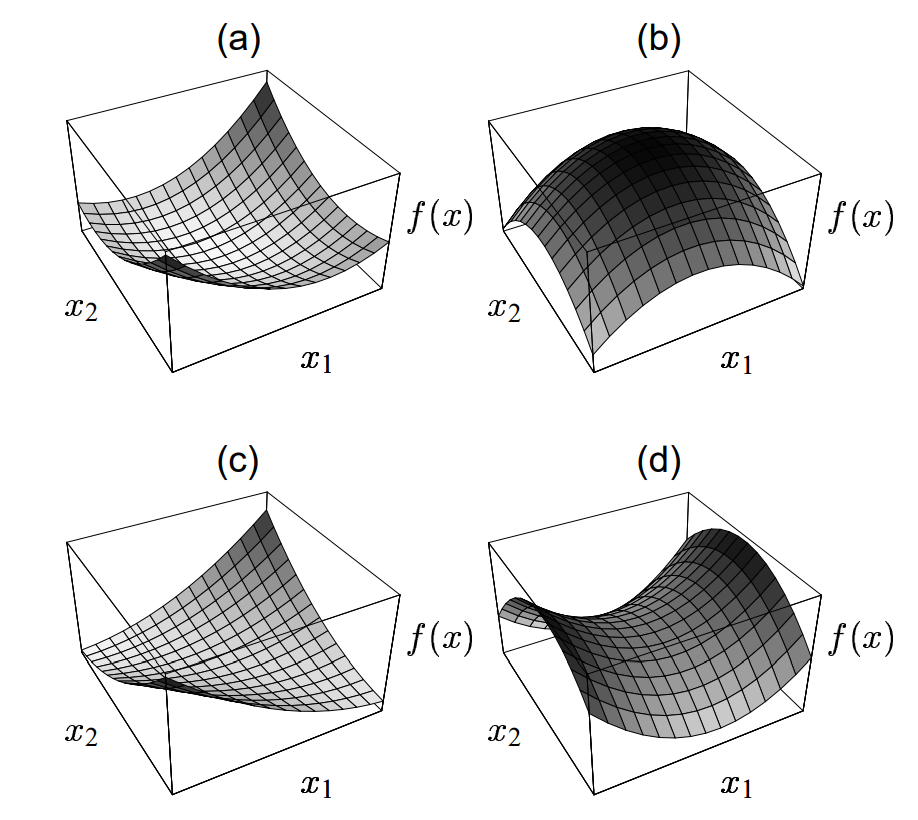
\includegraphics[scale=0.3]{figure/quadraticform.png}
   \caption{(a) Quadratic form for a positive-definite matrix. (b) For a negative-definite matrix. (c) For a singular (and positive-indefinite) matrix. A line that runs through the bottom of the valley is the set of solutions. (d) For an indefinite matrix. Because the solution is a saddle point, Steepest Descent and CG will not work. In three dimensions or higher, a singular matrix can also have a saddle.}
   \label{fig:quadratic}
\end{figure}


\section{Iterative Methods for Optimization}
\subsection{Steepest Descent Method}
In the method of steepest descent, we start at an arbitrary point $x_0$ and slide down to the bottom of the paraboloid. When we take a step, we choose the direction in which $f$ decreases most quickly, which is the direction $-\nabla f(x_i)= b-Ax_i$. 

For example, we will choose a point
\begin{equation}
    x_1=x_0+\alpha_0 r_0
\end{equation}

And the question is how big a step we should take? The line search is a procedure that chooses $\alpha$ to minimize $f$ along the line, as Figure \ref{fig:steepest}(c) shows. On the search line, $f$ is minimized where the gradient is orthogonal to the search line, then we know how to determine $\alpha$:
\begin{align*}
    r_{k+1}^Tr_k&=0\\
    (b-Ax_{k+1})^Tr_k&=0\\
    (b-A(x_k+\alpha_kr_k))^Tr_k&=0\\
    (b-Ax_k)^Tr_k-\alpha_k(Ar_k)^Tr_k&=0\\
    \alpha_k(Ar_k)^Tr_k&=(b-Ax_k)^Tr_k\\
    \alpha_kr_k^TAr_k&=r_k^Tr_k\\
    \alpha_k&=\boxed{\frac{r_k^Tr_k}{r_k^TAr_k}} \numberthis
\end{align*}

In summary, the whole process can be described below:
\begin{enumerate}
\item Set $k=0$, select an initial point $x_k\in\mathbb{R}^n$.
\item Set $r_k=b-Ax_k$. If $ r_k=0$, stop.
\item Update $\alpha_k=\frac{r_k^Tr_k}{r_k^TAr_k}$.
\item Update $x_{k+1}=x_k+\alpha_kr_k$.
\item Set $k=k+1$, then go to step 2.
\end{enumerate}

\begin{figure}[H]
   \centering
   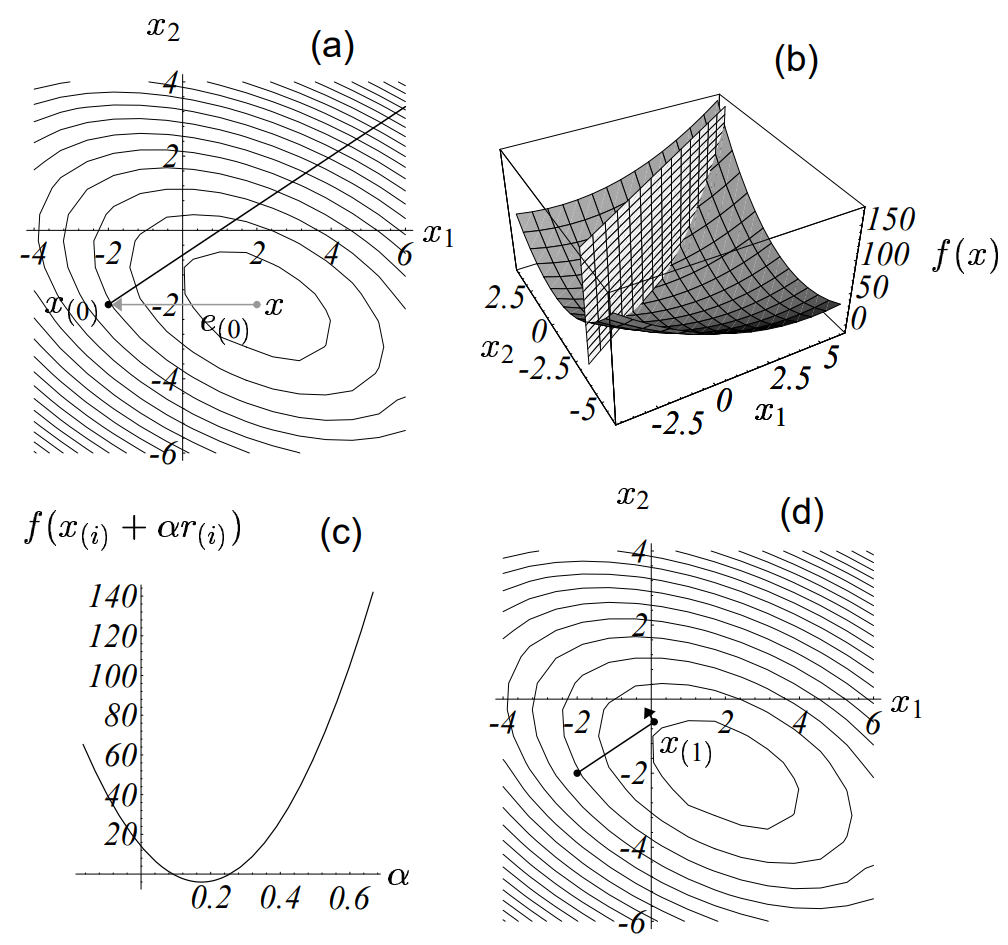
\includegraphics[scale=0.4]{figure/steepest_descent.png}
   \caption{The method of Steepest Descent. (a) Starting at $[-2,-2]^T$, take a step in the direction of steepest descent of $f$. (b) Find the point on the intersection of these two surfaces that minimizes $f$. (c) This parabola is the intersection of surfaces. The bottom most point is our target. (d) The gradient at the bottom most point is orthogonal to the gradient of the previous step.}
   \label{fig:steepest}
\end{figure}

\begin{figure}[H]
   \centering
   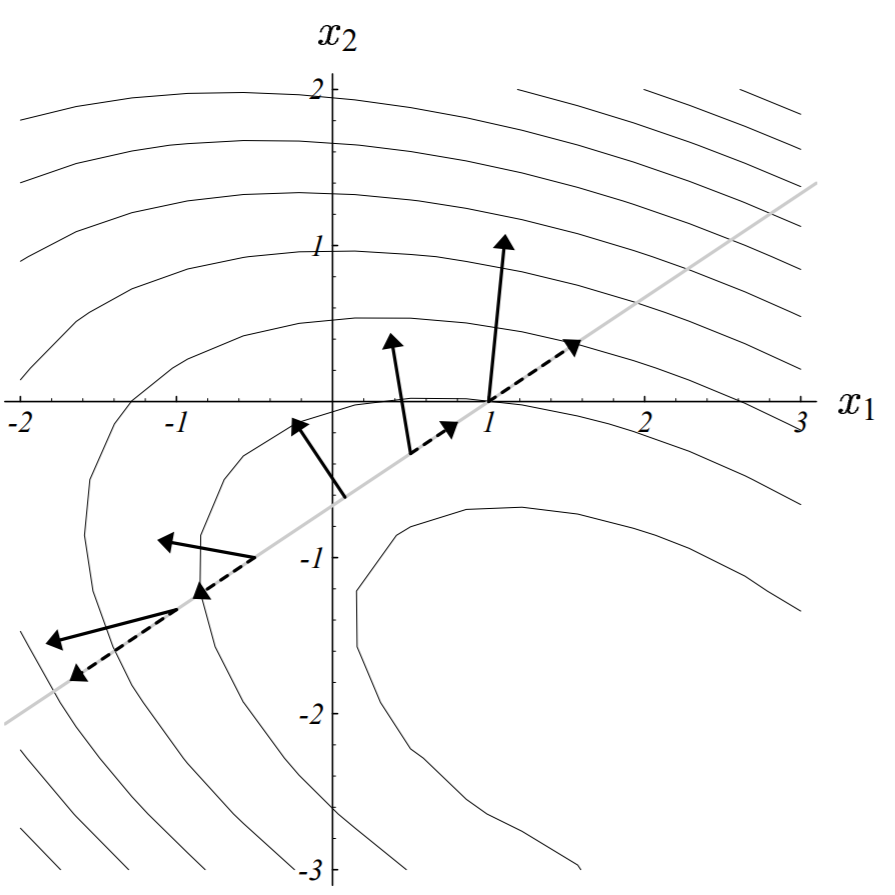
\includegraphics[scale=0.3]{figure/search_line.png}
   \caption{The gradient $\nabla f$ is shown at several locations along the search line (solid arrows). Each gradient’s projection onto the line is also shown (dotted arrows). The gradient vectors represent the direction of steepest ascent of $f$, and the projections represent the rate of increase as one traverses the search line. On the search line, $f$ is minimized where the gradient is orthogonal to the search line.}
   \label{fig:searchline}
\end{figure}

\subsection{Conjugate Gradient Method}

Steepest descent often finds itself taking steps in the same direction as earlier steps.  Wouldn’t it be better if, every time we took a step, we got it right the first time? Here’s an idea: let’s pick a set of orthogonal search directions $\{ p_1,  p_2,\cdots, p_n\}$. In each search direction, we’ll take exactly one step, and that step will be just the right length to line up evenly with $x_*$. After $n$ steps, we’ll be done.

And here comes the conjugate gradient method. Remember that for any starting point $x_0$, the conjugate gradient method converges to the unique minimum $x_*$ of $f$ in only $n$ steps. In our case, $n$ is the total number of pixels in the image. $A$ is a $n\times n$ symmetric and positive-definite matrix. Let $\{ p_1,  p_2,\cdots, p_n\}$ be $A$-conjugate vectors. (We cannot have more than $n$ linearly independent vectors in $\mathbb{R}^n$, hence we cannot have more than $n$ vectors that are $A$-conjugate. Plus, if $A=I$, then $\{ p_1,  p_2,\cdots, p_n\}$ are orthogonal vectors.) Since these vectors are independent, we can denote solution $ x_*$ with 
\begin{equation}
    x_*=x_0+\sum_{i=1}^n\alpha_i  p_i,
\end{equation}
where $\alpha_i$ is the step size along direction $ p_i$. 

Eq.\eqref{eq:x_update} is the update rule:
\begin{align*}
    x_{k+1}&=x_k+\alpha_k p_k \\ \numberthis \label{eq:x_update}
    x_{1}&=x_0+\alpha_0 p_0   \\ 
    x_{2}&=x_0+\alpha_0 p_0+\alpha_1 p_1 \\ 
    x_{k}&=x_0+\alpha_0 p_0+\cdots+\alpha_{k-1} p_{k-1} \\ 
    x_{*}&=x_{n}=x_0+\alpha_0 p_0+\cdots+\alpha_{n-1} p_{n-1}
\end{align*}

From Eq.\eqref{eq:x_update}, we can get
\begin{align}
    x_{k}-x_{0}&=\alpha_0 p_0+\cdots+\alpha_{k-1} p_{k-1}\\ \label{eq:xkx0}
    x_{*}-x_{0}&=\alpha_0 p_0+\cdots+\alpha_{n-1} p_{n-1}
\end{align}

 Since $ p_k$ is conjugate to each other, for every $k\not=i$, $ p_k^TA  p_i=0$. Times $ p_{k}^TA$ on both sides of Eq.\eqref{eq:xkx0}, we'll get
\begin{align}
     p_{k}^TA(x_{k}-x_{0})&= p_{k}^TA(\alpha_0 p_0+\cdots+\alpha_{k-1} p_{k-1})=0\\
     p_{k}^TA(x_{*}-x_{0})&= p_{k}^TA(\alpha_0 p_0+\cdots+\alpha_{n-1} p_{n-1})=\alpha_k p_{k}^TA p_{k}
\end{align}

From Eq.(11), we'll get
\begin{align}
    \alpha_k&=\frac{ p_{k}^TA(x_{*}-x_{0})}{ p_{k}^TA p_{k}}=\frac{ p_{k}^TA(x_{*}-x_{k}+x_{k}-x_{0})}{ p_{k}^TA p_{k}}
\end{align}

Take Eq.(10) into Eq.(12), we'll get
\begin{align*}
    \alpha_k&=\frac{ p_{k}^TA(x_{*}-x_{k})}{ p_{k}^TA p_{k}}\\ 
    &=\frac{ p_{k}^T(Ax_{*}-Ax_{k})}{ p_{k}^TA p_{k}}\\ 
    &=\frac{ p_{k}^T( b-Ax_{k})}{ p_{k}^TA p_{k}}\\ 
    &=\boxed{\frac{ p_{k}^T r_k}{ p_{k}^TA p_{k}}}\numberthis
\end{align*}

$ r_k$ is the negative gradient of $f$ at $x_k$, along which the steepest descent method would require to move. It can be updated by it's definition:
\begin{equation}
    r_k=\boxed{b-Ax_k}
\end{equation}

Or, it can just be updated by taking the relationship between $e$ and $r$, which is usually how we implemented in algorithm:
\begin{align*}
    x_{k+1}&=x_k+\alpha_kp_k\\ 
    x_{k+1}-x_*&=x_k-x_*+\alpha_kp_k\\ 
    e_{k+1}&=e_k+\alpha_kp_k\\ 
    -Ae_{k+1}&=-Ae_k-\alpha_kAp_k\\
    r_{k+1}&=\boxed{r_k-\alpha_kAp_k} \numberthis
\end{align*}

According to experiment, there's not much numerical difference between the above two update methods.
However, we are not doing steepest descent here, which may still have slight move on previous search directions $p$ and cause "zig-zag" path in descent. \textbf{The $\alpha_k$ above already tells us how long a step should take in the corresponding $p_k$ such that $p_k$ is conjugate to all the previous $p$,} and that is guaranteed by Eq.(10). 

Then the problem comes to how to determine $p_k$, and we give the following expression (imagine $\beta$ is a negative number, so it's just like subtracting conjugation from residual)
\begin{equation}
   \boxed{ p_k= r_k+\sum_{i<k}\beta_i p_i=r_k+\beta_{k-1}p_{k-1},}\text{  where $ p_0= r_0$.}
\end{equation}

 It's analogous to the usual Gram-Schmidt process for obtaining an orthogonal basis. \textbf{$\beta_i$ indicates the conjugate projection component on $p_i$.} The update rule for $p_k$ is that, in each iteration, the new conjugate direction is current negative gradient eliminated all the previous conjugate directions, as Figure~\ref{fig:gram} illustrates. 
 
 Since it's an iterative method, we only have to consider eliminating last search direction $p_{k-1}$ in term of conjugation. \textbf{Residual is orthogonal (error is conjugate) to all previous search directions}, which can be explained by derivation below:
 
 \begin{align*}
     e_k=x_k-x_*&=-\sum^n_{i=k}\alpha_ip_i\\
     p^T_jAe_k&=-\sum^n_{i=k}\alpha_ip_j^TAp_i &&\text{$j<k$}\\
     -p_j^Tr_k&=-\sum^n_{i=k}\alpha_ip_j^TAp_i\\
     p_j^Tr_k&=0\numberthis &&\text{$j\not=i$, then $p_i$ is conjugate to $p_j$}
 \end{align*}
 
 Also \textbf{residual is orthogonal (not conjugate) to all previous residuals}, which can be explained by derivation below:
 
 \begin{align*}
     p_k&=r_k+\sum_{i<k}\beta_ip_i\\
     r_j^Tp_k&=r_j^Tr_k+\sum_{i<k}\beta_ir_j^Tp_i &&\text{$k<j$}\\
     r_j^Tr_k&=0\numberthis &&\text{according to Eq.(17)}
 \end{align*}
 
 As each new search direction is constructed from the residual to be $A$-orthogonal to all the previous residual and search directions, the linear span of previous search directions and residual are identical. So comes from the above two conclusions.

\begin{figure}[H]
    \centering
    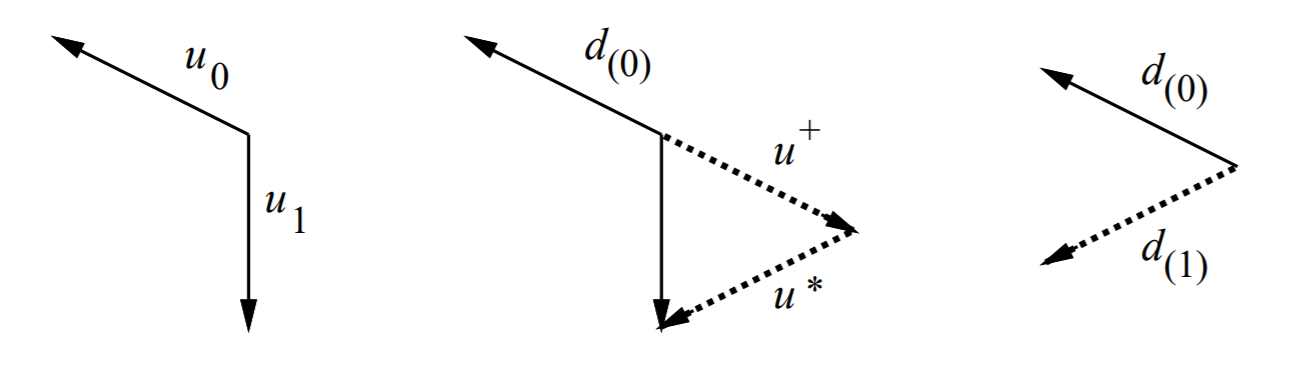
\includegraphics[scale=0.3]{figure/Gram-Schmidt_conjuga}
    \caption{Gram-Schmidt conjugation of two vectors. Begin with two linearly independent vectors $u_0$ and
$u_1$. Set $d_0=u_0$. The vector $u_1$ is composed of two components: $u^*$, which is conjugate to $d_0$ and $u^+$, which is parallel to $d_0$. After conjugation, only the $A$-orthogonal portion remains, and $d_1=u^*$. \textbf{If we stretch the space until the ellipses appeared circular, we'll find that $d_0$ and $d_1$ are strictly orthogonal.}}
    \label{fig:gram}
\end{figure}

Similar to the solution of $\alpha$, we use the conjugate property of $ p_i$ to calculate $\beta_k$. Times $ p_k^TA$ on both sides of Eq.(12), it goes to
\begin{align}
    p_k^TA p_{k+1}&= p_k^TA( r_{k+1}+\sum_{i<k+1}\beta_i p_i)\\
   0&= p_k^TA r_{k+1}+\sum_{i<k+1}\beta_i p_k^TA p_i\\
   0&= p_k^TA r_{k+1}+\beta_k p_k^TA p_k
\end{align}

From Eq.(19), we get the expression of $\beta$:
\begin{equation}
    \beta_k=\boxed{-\frac{ p_k^TA r_{k+1}}{ p_k^TA p_k}}
\end{equation}

Let us simplify this expression by taking the inner product of $r_k$ and Eq.(14):
\begin{align*}
    r_{k+1}^Tr_{k+1}&=r_{k+1}^Tr_k-\alpha_k r_{k+1}^TAp_k\\
    \alpha_k r_{k+1}^TAp_k&=r_{k+1}^Tr_k-r_{k+1}^Tr_{k+1}\\
    \alpha_k r_{k+1}^TAp_k&=-r_{k+1}^Tr_{k+1}\text{ (Each new residual is orthogonal to all the previous residuals.)}\\
     r_{k+1}^TAp_k&=-\frac{1}{\alpha_k}r_{k+1}^Tr_{k+1}\\
     p_k^TAr_{k+1}&=-\frac{1}{\alpha_k}r_{k+1}^Tr_{k+1}\numberthis\text{ ($A$ is symmetric.)}
\end{align*}

Therefore by substituting Eq.(12) and Eq.(20) into Eq.(19), $\beta$ can be simplified as
\begin{align*}
    \beta_k&=\frac{1}{\alpha_k}\frac{r_{k+1}^Tr_{k+1}}{ p_k^TA p_k}\\
    &=\frac{p_k^TAp_k}{p_k^Tr_k}\frac{r_{k+1}^Tr_{k+1}}{ p_k^TA p_k}\\
    &=\boxed{\frac{r_{k+1}^Tr_{k+1}}{p_k^Tr_k}}\numberthis
\end{align*}

With $x_k,\alpha_k\text{ and } p_k$, the update rule is as clear as
\begin{equation}
   x_{k+1}=x_k+\alpha_k p_k
\end{equation}

In summary, the whole process can be described below:
\begin{enumerate}
\item Set $k=0$, select an initial point $x_0\in\mathbb{R}^n$.
\item Set $r_0=-\nabla f(x_0), p_0= r_0$. If $ r_0=0$, stop.
\item Solve the step size along $p_k$: $\alpha_k=\frac{ p_{k}^T r_k}{ p_{k}^TA p_{k}}$.
\item Update the estimation with $\alpha_k, p_k$: $x_{k+1}=x_k+\alpha_k p_k$.
\item Set $ r_{k+1}=-\nabla f(x_{k+1})$ or $r_{k+1}=r_k-\alpha_kAp_k$. If $ r_{k+1}=0$, stop.
\item Solve the conjugation components among $r_k$: $\beta_k=\frac{r_{k+1}^Tr_{k+1}}{p_k^Tr_k}$.
\item Doing conjugation on $r_{k+1}$: $p_{k+1}= r_{k+1}+\beta_k p_k$.
\item Set $k=k+1$, then go to step 3.
\end{enumerate}

\subsection{Iterative Method}

The key to making progress is to note that in general, the matrix $A$ is extremely sparse, since the linear relationships usually only relate nearby grid points together. We therefore seek methods which don't require ever explicitly specifying all the elements of $A$, but exploit its special structure directly. Many of these methods are iterative - we start with a guess $x_k$, and apply a process that yields a closer solution $x_{k+1}$.

Let's recap the idea of Eigen first: $Ax=\lambda x$. If $|\lambda|<1$, then $A^iv=\lambda^iv$ will vanish as $i$ approaches infinity. If $|\lambda|>1$, then $A^iv$ will grow into infinity as $i$ approaches infinity.
\begin{figure}[H]
    \centering
    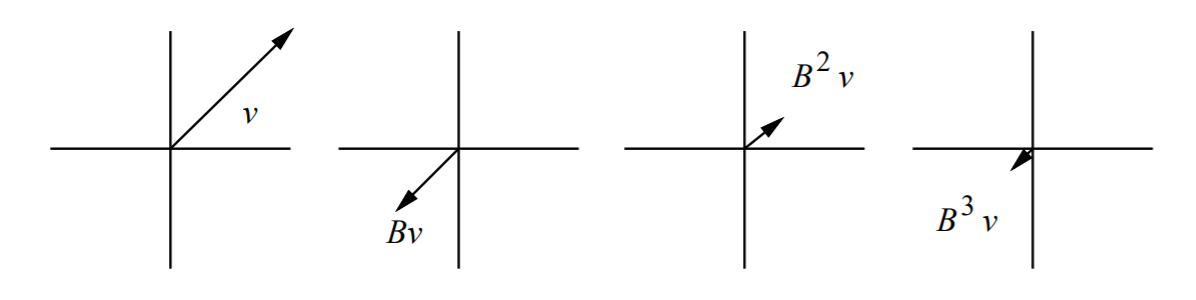
\includegraphics[scale=0.3]{figure/zero.png}
    \caption{As $i$ increases, $A^iv$ converges to zero with $|\lambda|<1$.}
\end{figure}
\begin{figure}[H]
    \centering
    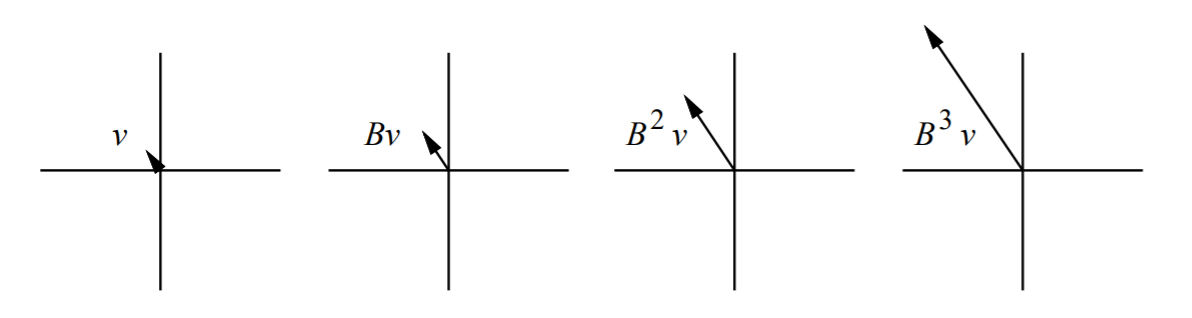
\includegraphics[scale=0.3]{figure/infinity.png}
    \caption{As $i$ increases, $A^iv$ diverges to infinity with $|\lambda|>1$.}
\end{figure}
A very important skill in understanding linear algebra is to think of a vector as a sum of other vectors whose behavior is understood. Say a vector $x$ is illustrated as a sum of two eigenvectors $v_1, v_2$. Applying $A$ to $x$ is equivalent to applying $A$ to the eigenvectors, and summing the result. 

On repeated application, we have $A^ix=A^iv_1+A^iv_2=\lambda^iv_1+\lambda^iv_2$. If the magnitudes of all the eigenvalues are smaller than 1, $A^ix$ will converge to 0, because the eigenvectors that compose $x$ converge to 0 when $A$ is repeatedly applied. If one of the eigenvalues has magnitude greater than 1, $x$ will diverge to infinity. This is why numerical analysts attach importance to the \textbf{spectral radius} of a matrix:
\begin{equation}
    \rho(R) = max{|\lambda_j|}\text{,  where the $\lambda_j$ are the eigenvalues of $R$}
\end{equation}
An iterative scheme converges if and only if $\rho(R)<1$. The size of the spectral radius determines the convergence rate, and ideally we would like to find splittings which result in as small a $\rho(R)$ as possible.

\paragraph{Jacobi Method.}The Jacobi method is one of the simplest iterations to implement. We split $A$ into $D+R$, where $D$ is the diagonal component and $R$ is the remainder. The convergence properties are then set by the matrix $D^{−1}R$.
\begin{align}
    Ax&= b \\ \nonumber
    (D+R)x&= b \\ \nonumber
    Dx&= b-Rx \\ \nonumber
    x^{(m+1)}&=D^{-1}( b-Rx^{(m)})
\end{align}
We start with an initial guess $x_0$, and then successively improve it according to Eq.(22). And entry-wise iteration is shown as below:
\begin{algorithm}
    \caption{Jacobi Method}
    \begin{algorithmic}
        \For{$j=1 \text{ to } N^2$}
        \State $x^{(m+1)}_j=\frac{1}{a_{jj}}(b_j-\sum_{k\not= j}a_{jk}x^{(m)}_k)$
        \EndFor
    \end{algorithmic}
\end{algorithm}
\\where $\frac{1}{a_{jj}},b_j,a_{jk}$ correspond to $D^{-1}, b, R$ respectively.
\\
\paragraph{Gauss-Seidel Method.} The Gauss–Seidel method improves on the Jacobi algorithm, by noting that if we are up-dating a particular point $u^{(m+1)}_j$, we might as well reference the already updated values $x^{(m+1)}_1,x^{(m+1)}_2,\dots,x^{(m+1)}_{j-1}$ in the calculation, rather than using the original values $x^{(m)}_1,x^{(m)}_2,\dots,x^{(m)}_{j-1}$. According to the property of Gauss-Seidel, we split $A$ into $L_*+U$, where $L_*$ is a lower triangular component and $U$ is a strictly upper triangular component.
\begin{align}
    Ax&= b \\ \nonumber
    (L_*+U)x&= b \\ \nonumber
    L_*x&= b-Ux \\ \nonumber
    x^{(m+1)}&=L_*^{-1}( b-Ux^{(m)})
\end{align}
The entry-wise iteration can be written as:
\begin{algorithm}
    \caption{Gauss-Seidel Method}
    \begin{algorithmic}
        \For{$j=1 \text{ to } N^2$}
        \State $x^{(m+1)}_j=\frac{1}{a_{jj}}(b_j-\sum_{k=1}^{j-1}a_{jk}x^{(m+1)}_k-\sum_{k= j+1}^{N^2}a_{jk}x^{(m)}_k)$
        \EndFor
    \end{algorithmic}
\end{algorithm}
\\
\paragraph{Multigrid Method.} This method is to make the progress converge faster on a final grid. The idea of multigrid is to take advantage of the fact that Jacobi and Gauss-Seidel method converge very fast on a coarse grid. And the effect of the iterations is essentially smoothing out the solution error. Initially, the solution error is the true solution itself. But over the iterations, the error gets way more smoother. The important steps are:
\begin{itemize}
    \item \textbf{Smoothing} – reducing high frequency errors, using a few iterations of the Jacobi or Gauss–Seidel method.
    \item \textbf{Residual Computation} – computing residual error after the smoothing operation(s).
    \item \textbf{Restriction} – downsampling the residual error to a coarser grid.
    \item \textbf{Interpolation} – interpolating a correction computed on a coarser grid into a finer grid.
    \item \textbf{Correction} – Adding prolongated coarser grid solution onto the finer grid.
\end{itemize}
Figure 1 and 2 shows the convergence of the conjugate gradient methods with and without preconditioner, respectively. On small size Lena, the CG method without preconditioner takes 54 iterations for residual's norm to reach below 10, while the one with preconditioning takes 22 interations. On large size Lena, the CG method without preconditioner takes 112 iterations for residual's norm to reach below 50, while the one with preconditioning takes only 87 interations.
\begin{figure}[H]
   \centering
   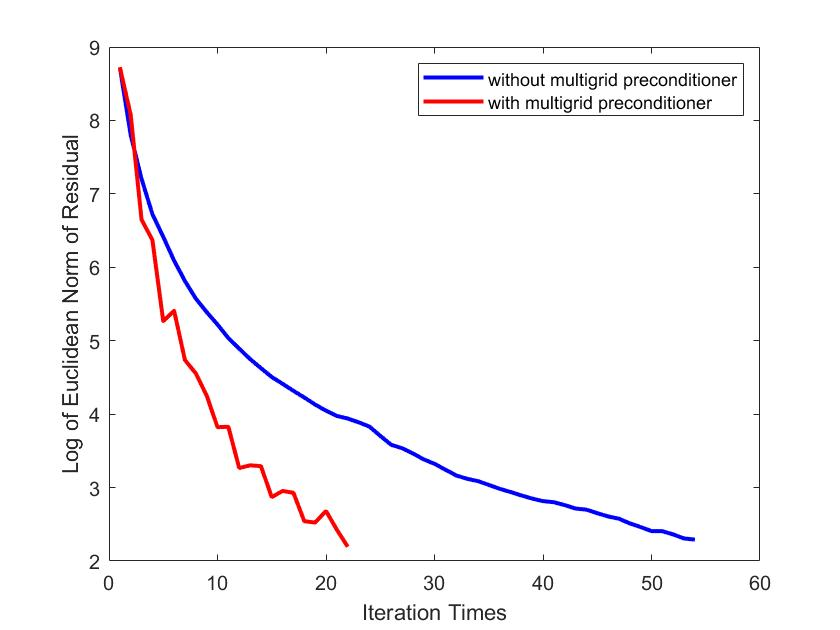
\includegraphics[scale=0.3]{figure/convergence_lena.jpg}
   \caption{The convergence on small size Lena.}
\end{figure}

\begin{figure}[H]
   \centering
   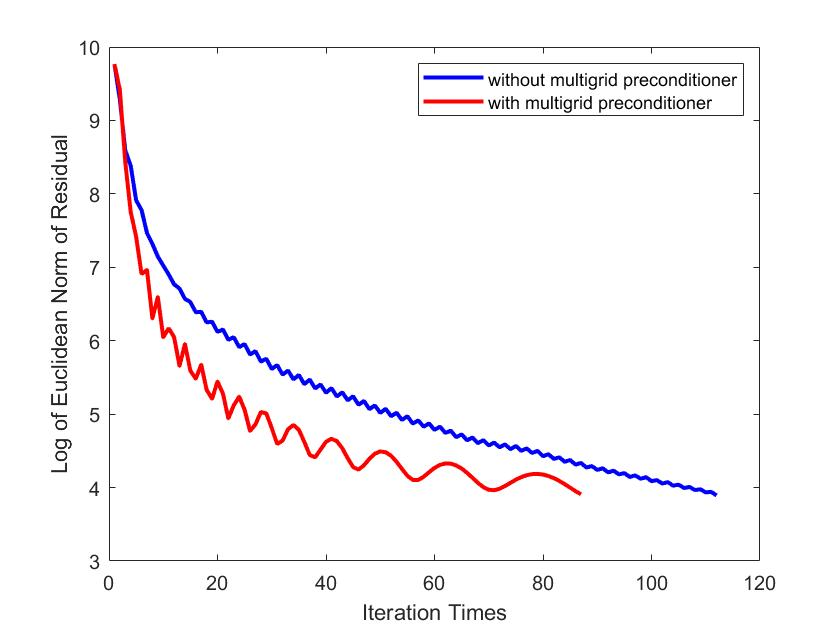
\includegraphics[scale=0.3]{figure/convergence_lenal.jpg}
   \caption{The convergence on large size Lena.}
\end{figure}

\section{Implementation}
\subsection{Conjugate Gradiant Method}
The $b$, $A$, $x_0$ here correspond to above $F$, $E$, $U$, respectively. And I initialize the $F$, $ g$ to Laplacian filtered $\textit{lena}$, all-one-matrix, respectively. The condition for stopping the iteration is $r_{k+1}<10$.

Figure 3 shows the result where $g(x,y)=x^2+y^2$. The progress takes 59 iterations in total.
\begin{figure}[H]
   \centering
   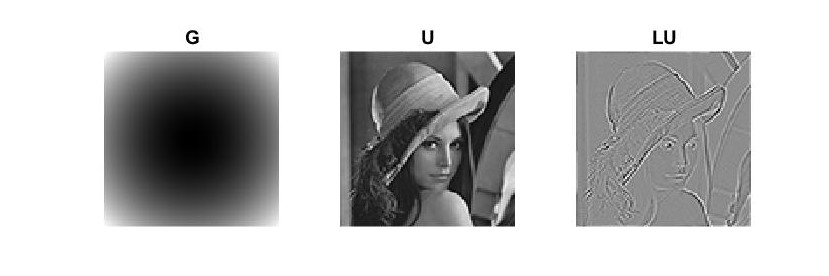
\includegraphics[scale=0.8]{figure/cg.jpg}
   \caption{From left to right: $G$, $U$, $F$.}
\end{figure}

\subsection{Iterative Method}
Below is my implementation of multigrid method. As a preconditioner, the multigrid works just like $z_1=M^{-1}r_1$, so the multigrid function should be called like $z_1=multigrid(0,r_1)$.
\begin{algorithm}  [H]
\caption{Multigrid}\label{algo1}
    \begin{algorithmic}
            \Function{multigrid}{$x_0,b$}
                
                \For{$i=[1:10]$}
                    \State $x_0=jacobi(x_0,b)$ \Comment{Smoothing}
                \EndFor
                \State $residual = Ax-b$ \Comment{Residual Computation}
                \State $residual\_coarse=sample(residual)$ \Comment{Restriction}
                \If{$size(b,1)>1$}
                    \State $error\_coarse = multigrid(error\_coarse, residual\_coarse)$
                \EndIf
                \State $error=interpolate(error\_coarse)$ \Comment{Interpolation}
                \State $x=x_0-error$ \Comment{Correction}
                \State \Return{$x$}
            \EndFunction
        \end{algorithmic}  
\end{algorithm} 
Figure 4 shows the result of multigrid precondtioned congjugate gradient methond.
\begin{figure}[H]
   \centering
   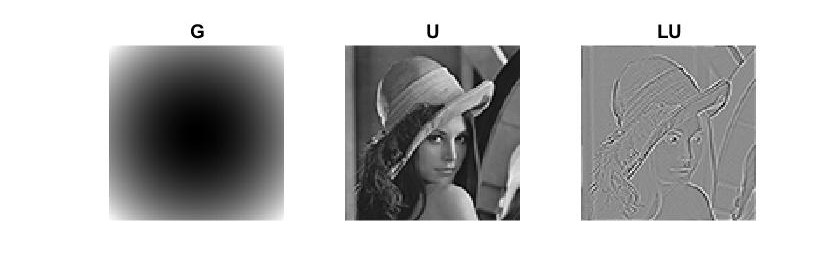
\includegraphics[scale=0.8]{figure/cgmg.jpg}
   \caption{From left to right: $G$, $U$, $F$.}
\end{figure}

\newpage
\end{document}
